\chapter{Asking Palm Beach Billionaires How They Got So Rich}

This chapter is best read as a field lecture rather than a classroom lecture. We begin with spectacle, move through the problem of access, and then extract from several short interviews a compact commercial mathematics: the arithmetic of scale, retention, leverage, negotiation, and demand. No validated board screenshot survives for this lecture, so whenever we write an equation or draw a figure, it is a careful transcript-led reconstruction rather than a transcription from a blackboard.

\section{Palm Beach as a Private Wealth Field}

The lecture opens with a teaser montage of strange and oversized claims: a bizarre career path, a billion-dollar business, a few hundred million in a year, a large legal resolution. Only after this does the host reset the frame. We are in West Palm Beach, or Palm Beach more loosely, and the governing question is how people here got rich.

\paragraph{Claim.} The city-scale numerical anchor matters because it explains the tone of the whole lecture: this is not a generic street interview, but a hunt inside a dense field of visible wealth.
\begin{align}
N_{\mathrm{billionaires}} &> 60,\\
F_{\mathrm{host},1} &\approx 12.7\times 10^6,\\
F_{\mathrm{host},2} &\approx 5.4\times 10^6.
\end{align}
The first number is the host's stated billionaire count; the next two are host-stated audience sizes used as access credentials. The point is not that these numbers prove business truth. The point is that, in this lecture, access itself has a structure.

\paragraph{Mechanism.} The early refusals show us the first recurrence. The wealthy pedestrian is private, skeptical, and in motion; the interviewer counters with persistence, brevity, and legitimacy. The lecture therefore begins with a kind of access funnel.

\begin{figure}[h]
\centering
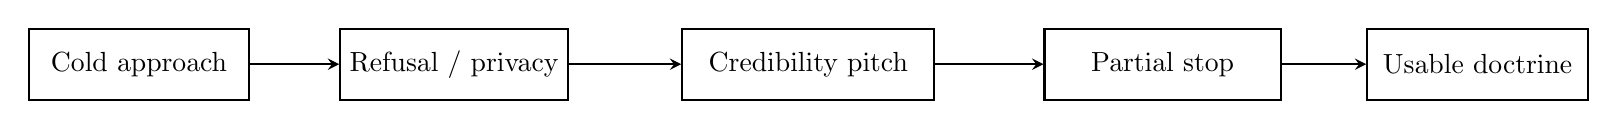
\begin{tikzpicture}[>=stealth, thick]
\node[draw, rectangle, minimum width=2.8cm, minimum height=0.9cm] (a) at (0,0) {Cold approach};
\node[draw, rectangle, minimum width=2.8cm, minimum height=0.9cm] (b) at (4,0) {Refusal / privacy};
\node[draw, rectangle, minimum width=3.2cm, minimum height=0.9cm] (c) at (8.5,0) {Credibility pitch};
\node[draw, rectangle, minimum width=3.0cm, minimum height=0.9cm] (d) at (13,0) {Partial stop};
\node[draw, rectangle, minimum width=2.8cm, minimum height=0.9cm] (e) at (17,0) {Usable doctrine};
\draw[->] (a) -- (b);
\draw[->] (b) -- (c);
\draw[->] (c) -- (d);
\draw[->] (d) -- (e);
\end{tikzpicture}
\caption{Transcript-derived access funnel: the lecture first solves the problem of contact, and only then extracts doctrine.}
\end{figure}

\subsection{Question \& Answer}

\paragraph{Question.} Why does ``no'' not mean ``never'' in this lecture?

\paragraph{Answer.} Because the initial ``no'' is not presented as a logical refutation of the project. It is presented as the ambient friction of a privacy-heavy environment. The host's motto, ``no does not mean never; it means not yet,'' is therefore not motivational ornament. It is a practical statement about repeated contact in a field where wealth and privacy are positively correlated.

\section{From Rooftop Gravel to a Nationwide Vacuum-Truck Business}

The first substantial case is also the cleanest entrepreneurial arc. One speaker says that after college he got behind the wheel of a truck and sucked gravel off rooftops. From there he moved into industrial cleaning for power plants, refineries, and steel mills, and from there into a nationwide vacuum-truck business and a liquid storage tank business.

\paragraph{Anecdote.} The lecture wants us to keep the oddity of the starting point. This is not a smooth managerial ascent. It is a manual niche that becomes an industrial niche and only then becomes a scalable service platform.

\paragraph{Claim.} Two operating rules appear immediately: sales were done by knocking on doors cold, and the business was started with no outside money.
\begin{align}
C_{\mathrm{truck},0} &= \$180{,}000,\\
C_{\mathrm{truck},\mathrm{now}} &\approx \$500{,}000\text{--}\$600{,}000.
\end{align}
The first truck is the lecture's clearest asset-cost anchor. It is also what lets the story move from effort to equipment.

\paragraph{Mechanism.} The speaker describes growth as entirely organic: profits are put back into the business. A cautious compact version is
\begin{equation}
K_{t+1}=K_t+\pi_t^{\mathrm{retained}},
\end{equation}
where \(K_t\) is productive operating capital and \(\pi_t^{\mathrm{retained}}\) is profit retained for reinvestment. We should not oversell this as a full accounting identity; it is merely the cleanest way to summarize the spoken mechanism.

The same speaker gives a quasi-diagrammatic rule for scale:
\begin{equation}
0 \not\to 100,\qquad 0 \to 5 \to 10 \to 15.
\end{equation}
The point is not the exact sequence of numbers. The point is that scale is staged. One does not leap over intermediate forms of competence.

A later durability marker sharpens the picture:
\begin{equation}
\frac{N_{\mathrm{closed\ offices}}}{N_{\mathrm{offices}}}=\frac{1}{40}.
\end{equation}
This is an unusually compact summary of survival: the business expanded, but it did not churn itself to death.

\subsection{Question \& Answer}

\paragraph{Question.} How does a business scale from zero without raising outside money?

\paragraph{Answer.} In the lecture, it scales by a loop, not by a jump.

\begin{enumerate}
\item Save enough cash to acquire the first productive asset.
\item Use that asset to perform a specialized task that customers already pay for.
\item Retain operating profit rather than extracting it.
\item Reinvest retained profit into more capacity, more geography, or more service lines.
\item Repeat until the business has a footprint larger than the founding asset.
\end{enumerate}

This is why the lecture pairs patience with passion. If the loop takes years, then internal motivation is not sentiment; it is a financing condition.

\section{Mortgage Timing, Plaintiff Law, and the Discoverability Pivot}

The next stretch broadens the lecture from industrial service into professional service. One speaker says he made his first million at \(25\) in mortgage banking in San Francisco, because real estate in California, and especially San Francisco, was booming. The route is plainly opportunistic in the literal sense: one stands where the price action is.

A second speaker, a personal-injury and mass-tort lawyer, says the legal business made him the most money and gives the lecture's clearest legal money markers:
\begin{align}
S_{\mathrm{case}} &= \$54\,\mathrm{M},\\
S_0 &= \$30\,\mathrm{M},\\
S_1 &> \$50\,\mathrm{M}.
\end{align}
These are case-resolution figures. We should not silently relabel them as law-firm revenue, fees, or personal income.

\paragraph{Claim.} In the law segment the lecture turns from sector timing to discoverability. The speaker says that early SEO worked because he was ahead of the market; later he says SEO is largely dead and that social media is now the better attention surface. The logic is stable even if the channel changes: competence without discoverability is commercially incomplete.

\paragraph{Mechanism.} The other mechanism in this section is team selection. When the lawyer says that the goal is to be the dumbest person in the room, he is offering a rule for wealth preservation as well as wealth creation. Stronger specialists stabilize capital after it has been accumulated.

\subsection{Question \& Answer}

\paragraph{Question.} Why leave \(\$30\,\mathrm{M}\) on the table?

\paragraph{Answer.} Because in the lecture the larger decision variable is not present comfort but eventual outcome. The worked example is simple:
\begin{align}
S_1-S_0 &> \$20\,\mathrm{M},\\
S_1 &> S_0.
\end{align}
The interviewee's rule is therefore: do not be prepared to do the deal at the table; be prepared to do the deal outside the room. In this specific case, delay strictly dominated immediate settlement.

\begin{enumerate}
\item A very large present offer appears.
\item The negotiator refuses to treat largeness as finality.
\item The case remains alive.
\item Time and bargaining pressure continue to work.
\item The later settlement exceeds the earlier one.
\end{enumerate}

The lecture does not generalize this into a theorem valid for every case. It gives it instead as a disciplined example of long-game negotiation.

\section{The Corporate Ladder as a Wealth Path}

After the founder-owner cases, the lecture deliberately changes texture. A public-company CEO, who says he spent his entire career at one business-services company, provides the non-founder route to large-scale wealth and authority. Here the business is not built from scratch by the interviewee; it is climbed from within.

\paragraph{Claim.} The corporate path matters because it prevents the chapter from collapsing wealth into one archetype. The lecture explicitly allows a second route: institutional ascent inside a sufficiently strong firm.

The scale markers are large:
\begin{align}
N_{\mathrm{employees}} &= 42{,}000,\\
T_{\mathrm{CEO}} &= 18\ \mathrm{years},\\
g_{\mathrm{rev}} &\in \text{high single digits.}
\end{align}
The company is described as doing multi-billions in annual revenue and maintaining that growth profile for fifty years. Whether or not the speaker reveals the company name, the scale logic is clear.

\subsection{Question \& Answer}

\paragraph{Question.} How does someone work up to CEO inside a giant company?

\paragraph{Answer.} The lecture's answer is strikingly procedural.

\begin{enumerate}
\item Finish the assigned work for the day.
\item Ask the boss what else needs to be done.
\item Take on tasks that would otherwise remain with the boss.
\item Learn the next layer of responsibility by doing those tasks.
\item Become legible as the boss's right-hand person.
\item When a larger role opens, be the person already associated with extra capacity.
\item Perform well at the higher level and repeat.
\end{enumerate}

This is not glamorous, but the lecture does not present it as glamorous. It presents it as cumulative.

\section{Pressure, Responsibility, and the Frog-in-the-Kettle Rule}

The natural next question is not how the climb happens, but what it feels like once it happens. The host presses on the problem of scale: shareholders, employees, customers, and performance pressure all sit on the executive at once. The answer is not that pressure disappears, but that tolerance changes.

\paragraph{Mechanism.} A cautious transcript-derived schematic is
\begin{equation}
P_{t+1}>P_t,\qquad \Theta_{t+1}>\Theta_t,
\end{equation}
where \(P_t\) denotes role pressure and \(\Theta_t\) denotes tolerance to it. This is not a measured law. It is the closest mathematical restatement of the speaker's frog-in-the-kettle analogy.

\begin{enumerate}
\item Responsibility rises with advancement.
\item Harder problems appear at each new level.
\item Repeated exposure reduces the tendency to overreact.
\item One therefore carries more pressure because one has slowly become able to carry more pressure.
\end{enumerate}

\paragraph{Remark.} The lecture pairs this acclimation rule with a darker corporate realism: a business career contains more problems than upside moments. That line is slightly garbled in the transcript, but its meaning is clear. The point of executive maturity is not to abolish hard problems. It is to metabolize them.

\section{AI Infrastructure, Diversification, and Relationship Selling}

After a brief online-presence interlude, the lecture re-enters through physical infrastructure. One interviewee, whose business sells generators and heavy equipment, says he made his first million at \(42\), that his current business is around a billion in scale, that he once had roughly \(\$500\,\mathrm{M}\) of order intake in a year, and that his largest single-customer order was around \(\$250\,\mathrm{M}\).

\paragraph{Claim.} The conceptual pivot is important. AI is not treated here as software cleverness but as a demand shock for electricity, data centers, standby power, and therefore industrial equipment.

The speaker's explicit heuristic is
\begin{equation}
\frac{L_{\mathrm{AI\ search}}}{L_{\mathrm{Google\ search}}}\approx 10.
\end{equation}
Again, we should preserve this as a speaker-attributed rule of thumb, not as an audited engineering constant. Its structural use is what matters.

\subsection{Question \& Answer}

\paragraph{Question.} How does AI make money for a company that is not itself an AI company?

\paragraph{Answer.} The lecture gives a short causal chain.
\begin{equation}
L_{\mathrm{AI\ load}}\uparrow \;\Rightarrow\; P_{\mathrm{data\ center}}\uparrow \;\Rightarrow\; Q_{\mathrm{generator}}\uparrow.
\end{equation}

\begin{enumerate}
\item AI-style queries require heavier compute than ordinary search.
\item Heavier compute raises data-center load.
\item Higher load raises both baseload and standby-power demand.
\item Generator suppliers therefore benefit even though they are not themselves AI firms.
\end{enumerate}

\paragraph{Mechanism.} The rest of the interview adds two stabilizers. First, diversification: the speaker says he has both geographical diversity and sector diversity. Second, relationship selling: a quarter-billion-dollar order is not closed by product specification alone. It is closed by trust, reassurance, and adaptation to customer type. The lecture insists on this social detail because the largest transactions are not merely technical allocations; they are acts of confidence.

\section{Private Equity, Leverage, and the Velocity of Cash}

The final interview is the lecture's most explicit capital-structure lesson. The speaker, now in private equity after earlier ventures in printing, display, and carton businesses, says that in today's world he would rather buy a business than start one. The reason is not abstract preference but financing structure: a business with a track record can borrow.

\paragraph{Claim.} The private-equity model is given in plain speech: buy a company, borrow against its assets, and pay that borrowing down through the company's cash flow. A cautious schematic version is
\begin{align}
D_t &\le A_t,\\
CF_t &\ge DS_t.
\end{align}
Here \(A_t\) is the acquired asset base, \(D_t\) the debt raised against it, \(CF_t\) the operating cash flow, and \(DS_t\) the debt-service burden. The lecture does not present these symbols, but it clearly presents the structure they describe.

\begin{figure}[h]
\centering
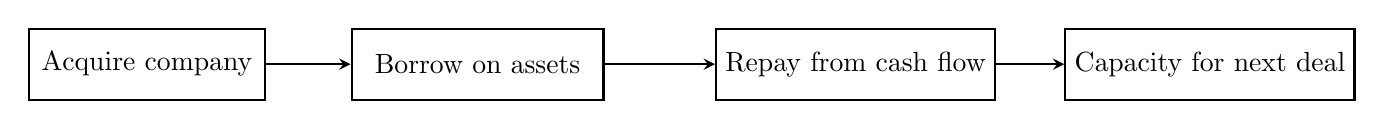
\begin{tikzpicture}[>=stealth, thick]
\node[draw, rectangle, minimum width=3.0cm, minimum height=0.9cm] (a) at (0,0) {Acquire company};
\node[draw, rectangle, minimum width=3.2cm, minimum height=0.9cm] (b) at (4.2,0) {Borrow on assets};
\node[draw, rectangle, minimum width=3.4cm, minimum height=0.9cm] (c) at (9.0,0) {Repay from cash flow};
\node[draw, rectangle, minimum width=3.0cm, minimum height=0.9cm] (d) at (13.5,0) {Capacity for next deal};
\draw[->] (a) -- (b);
\draw[->] (b) -- (c);
\draw[->] (c) -- (d);
\end{tikzpicture}
\caption{Transcript-derived private-equity loop.}
\end{figure}

\subsection{Question \& Answer}

\paragraph{Question.} What makes private equity work, and why is buying often easier than starting?

\paragraph{Answer.} In the lecture, buying is easier because the target business already has a record legible to banks. That legibility is itself a form of capital.

\begin{enumerate}
\item The acquired business has assets.
\item The acquired business has cash flow.
\item The bank can therefore lend against something already operating.
\item Debt can then be serviced by the business rather than solely by founder optimism.
\item Repaid debt and accumulated credibility support the next transaction.
\end{enumerate}

\paragraph{Mechanism.} The final mathematical idea is the distinction between margin and velocity of cash. The interviewee invokes Walmart: small margin, fast turns, large aggregate profit. A compact summary is
\begin{equation}
\Pi_{\mathrm{period}} \propto m\cdot v,
\end{equation}
where \(m\) is margin per turn and \(v\) is the number of turns per period. This is not a full profit formula; it is the lecture's way of warning us not to confuse thin margin with weak business quality.

The same speaker closes on two final principles. First, very successful people are usually willing to take risk; his own example is leveraging his house in an early acquisition. Second, the present directional thesis is U.S.\ manufacturing and onshoring. That is not proved in the lecture, but it is offered as a concluding investment judgment by a private-equity operator.

\section{Summary}

The lecture begins as a hunt and ends as a compact theory of how wealth is built under very different institutional forms. We see one route through manual niche work, retained earnings, and gradual asset accumulation; another through visibility, professional leverage, and patient negotiation; another through corporate ascent and the slow acquisition of responsibility; another through AI-driven infrastructure demand; and a final one through acquisition, leverage, and cash-flow discipline. What the interviews do not reduce is precisely what makes them useful: wealth is not one formula. But the lecture does leave us with a common backbone of recurrences---ownership, patience, trust, repeated reinvestment, and the willingness to let time, rather than appetite, govern the large decision.